\documentclass[11pt]{article}
\pdftrailerid{}
\usepackage{tikz}
\usepackage[T1]{fontenc}
\usepackage{lmodern}
\usepackage[a4paper,margin=24mm]{geometry}
\usepackage{amsmath,amssymb,amsthm,mathtools,microtype}
\usepackage{xcolor,xurl}
\usepackage[colorlinks=true,linkcolor=blue!50!black,urlcolor=blue!50!black,citecolor=blue!50!black]{hyperref}
\renewcommand{\abstractname}{Resumen}
\renewcommand{\proofname}{Demostración}
\renewcommand{\refname}{Referencias}
\renewcommand{\figurename}{Figura}
\DeclareMathOperator{\spanof}{span}
\newtheorem{theorem}{Teorema}
\newtheorem{corollary}[theorem]{Corolario}
\newtheorem{lemma}[theorem]{Lema}
\title{Recoloreo ponderado de aristas y 1-factorización a través de un corte}
\author{Juan Pablo Traverso Gianini\\\small Investigador independiente, Santiago, Chile\\\small\href{mailto:jtraverso@gmail.com}{jtraverso@gmail.com}\quad\href{https://orcid.org/0009-0003-6068-4096}{ORCID 0009-0003-6068-4096}}
\date{Preprint 1.0 · 24 de noviembre de 2026 · \mbox{\href{https://doi.org/10.5281/zenodo.24521352}{DOI 10.5281/zenodo.24521352}}}
\hypersetup{pdftitle={Recoloreo ponderado de aristas y 1-factorización a través de un corte},pdfauthor={Juan Pablo Traverso Gianini},pdfsubject={Preprint 1.0, DOI 10.5281/zenodo.24521352}}
\begin{document}
\maketitle

\begin{abstract}
Para completar un coloreo interno de aristas a través de un corte equilibrado hay que dejar suficientes copias cruzadas para cada color, en especial en los vértices con pocos vecinos ordinarios distintos. Demostramos una cota de recoloreo ponderado que conserva el tamaño prescrito de cada clase. Para tamaños iguales, la cota escalar es aguda y el orden óptimo para pesos vectoriales es la raíz cuadrada de la dimensión del espacio generado por los pesos centrados. Las reservas ponderadas de Hall permiten tratar varios vértices excepcionales a la vez. Al dividir los vértices ordinarios en bloques, la mayor violación de una desigualdad de corte da el déficit exacto del emparejamiento bajo una hipótesis de anchura. Cada color alcanza su déficit con copias disjuntas. Damos también un criterio de 1-factorización que combina las reservas de los excepcionales con un \emph{nibble} hipergáfico y una reparación simultánea en una reserva espectral. Una familia regular de rejillas tiene \(\Theta(\sqrt N)\) vecinos ordinarios cruzados distintos por vértice ordinario y \(\Theta(N^{1/4})\) excepcionales por lado, donde \(N\) es el número de ordinarios por lado. Una construcción directa factoriza la familia a partir de un umbral explícito, aunque el criterio de rectángulos falla en el corte dado para toda paleta admisible.
\end{abstract}

\section{Introducción}

Los coloreos internos y los emparejamientos cruzados de Shan~\cite{Shan} y de Chen, McDonald y Shan~\cite{CMS} sugieren el siguiente método para un multigrafo regular de orden par. Dividimos sus vértices en dos partes iguales, coloreamos las aristas de los subgrafos inducidos y completamos cada color interno a un emparejamiento perfecto mediante aristas cruzadas. El multigrafo residual es regular y bipartito. Si las dos clases internas de cada color tienen el mismo tamaño, quedan tantos vértices libres de un lado como del otro. También importa \emph{cuáles} quedan libres, especialmente cuando un vértice tiene pocos vecinos cruzados distintos y sus aristas tienen gran multiplicidad.

Para un vértice excepcional \(x\), un emparejamiento interno del lado opuesto cubre un conjunto \(U\) de vértices. Exactamente \(\sum_{v\in U}\mu(x,v)\) copias cruzadas de \(x\) terminan en \(U\), donde \(\mu(x,v)\) denota la multiplicidad. Este conteo sugiere asignar un peso a cada vértice y preguntar cuánto peso cubre cada color. Con varios excepcionales, cada \(v\) lleva una coordenada por cada \(x\). Cambiar una clase de color cambia todas esas sumas a la vez.

Partimos de una cota escalar de recoloreo para tamaños de clase prescritos. La Sección~\ref{sec:weights} da la prueba y un grafo conexo que alcanza la cota para tamaños iguales. El Teorema~\ref{thm:balance} también trata pesos vectoriales. Su cota depende de la dimensión del espacio generado por los pesos centrados, que puede ser mucho menor que el número de excepcionales. En la Sección~\ref{sec:cross} usamos cada coordenada para contar el peso que queda disponible para un vértice excepcional. Asignar a un par cruzado un peso menor que su multiplicidad resulta útil cuando varios excepcionales comparten un vecino. Las desigualdades resultantes dan tres condiciones suficientes para completar los colores uno a uno (Teorema~\ref{thm:factor}).

Las mismas reservas ponderadas dan dos resultados de completación. Si dividimos los ordinarios en bloques, los dos lados pueden tener el mismo total de libres para un color y cantidades distintas en cada bloque. El Teorema~\ref{thm:block-deficit} identifica el déficit exacto a partir de las asignaciones elegibles de los excepcionales y muestra que cada color alcanza su déficit con copias cruzadas disjuntas. El Teorema~\ref{thm:hybrid-completion} trata la competencia por copias entre colores. Tras emparejar a los excepcionales, usa un conjunto de copias ordinarias para obtener emparejamientos parciales de toda la paleta y un segundo conjunto para repararlos. La rejilla de la Sección~\ref{sec:sparse-reserve-example} ilustra el criterio. Sus copias de relleno también dan una construcción directa con umbral explícito en un corte donde la prueba de rectángulos falla para toda paleta admisible.

\subsection*{Relación con trabajos previos}

Los coloreos equitativos de aristas equilibran el número de aristas por clase de color \cite{McDiarmid,CariolaroFu}. Para grafos bipartitos, en la Sección~\ref{sec:weights} deducimos una cota escalar para tamaños equitativos del lema de Nash-Williams sobre dos familias laminares~\cite{NashWilliams}. El Teorema~\ref{thm:balance} prescribe el tamaño de cada clase y admite ciclos impares. Balister, Kostochka, Li y Schelp usan caminos alternantes y un potencial cuadrático para equilibrar las cantidades de vértices con paletas prescritas \cite{BKLS}. Shioura y Yagiura equilibran conteos de aristas globalmente y en pares paralelos \cite{SY}. Gajjala y Khan~\cite{GK} imponen una capacidad en cada vértice y color. Aquí la carga es la suma de los pesos de los vértices de todo el emparejamiento.

La construcción del corte parte de los argumentos de factorización de Shan y de Chen, McDonald y Shan \cite{Shan,CMS}. Nuestras hipótesis se refieren a un corte dado y permiten que varios excepcionales compartan vecinos de gran multiplicidad. La Sección~\ref{sec:two-fifths} compara los grados de una familia con los de resultados previos. En el ámbito espectral, Ferber y colaboradores obtienen un \(f\)-factor después de borrados acotados bajo una hipótesis sobre el grafo ambiente \cite[Lema~4.5]{FFMYZ}. La matriz del Teorema~\ref{thm:factor} mide el soporte simple entre ordinarios del corte prescrito. Las condiciones de corte por bloques usan el teorema de flujo entero de Gale~\cite{Gale} para determinar hasta dónde llega la completación ponderada de Hall después de que los colores anteriores han gastado copias.

Para la completación simultánea usamos la estimación del \emph{nibble} de Keevash, derivada del trabajo de Ehard, Glock y Joos~\cite{KeevashII,EGJ}. Broder, Frieze y Upfal~\cite{BFU} combinan recorridos de mezcla rápida y el lema local de Lovász para conectar pares prescritos en un expansor. En el Lema~\ref{lem:spectral-repair}, el emparejamiento actual determina los pasos hacia atrás de cada color. Contamos el uso de cada copia de reserva a lo largo de toda la paleta y el de cada arista del emparejamiento anterior dentro de su color. Las aristas paralelas del multigrafo se tratan como copias distintas.

\section{Recoloreo con tamaños de clase prescritos}\label{sec:weights}

Todos los multigrafos son finitos y sin lazos. Contamos las aristas paralelas con multiplicidad y distinguimos sus copias. Para un coloreo propio de aristas \(M_1,\ldots,M_k\) y una función de pesos \(w\) sobre los vértices, escribimos
\[
  m_i=|M_i|,\qquad W_i=\sum_{uv\in M_i}\bigl(w(u)+w(v)\bigr).
\]
Como cada \(M_i\) es un emparejamiento, \(W_i\) suma los pesos de los vértices que cubre.

\begin{theorem}\label{thm:balance}
Supongamos que \(G\) admite un coloreo propio de aristas con tamaños de clase \(m_1,\ldots,m_k\). Sea \(w\) una función con valores en un espacio euclidiano real de dimensión finita. Fijemos \(c\) y \(R\ge0\) con \(\|w(v)-c\|_2\le R\) para todo \(v\), y pongamos \(s=\dim\spanof\{w(v)-c:v\in V(G)\}\). Existe un coloreo propio de aristas en el que el color \(i\) conserva su tamaño \(m_i\) para cada \(i\) y, para todo \(i,j\), se cumple
\[
  \|(W_i-2m_i c)-(W_j-2m_j c)\|_2
  \le 2R\,\psi_s(|m_i-m_j|),
\]
donde
\[
 \psi_s(d)=
 \begin{cases}
   0 & s=0,\\
   2 & s=1,\ d=0,\\
   d & s=1,\ d>0,\\
   \sqrt{d^2+4s} & s\ge2.
 \end{cases}
\]
\end{theorem}

\begin{proof}
Escribimos \(z(v)=w(v)-c\) y \(Z_i=W_i-2m_i c\). Para \(s=0\) el resultado es inmediato. En el conjunto finito de coloreos con los tamaños dados, minimizamos \(\sum_i\|Z_i\|_2^2\). Fijamos dos colores distintos \(i,j\) con \(d=m_i-m_j\ge0\) y consideramos las componentes con aristas en el subgrafo de esos colores. Son caminos alternantes y ciclos pares, contando dos aristas paralelas como un ciclo de longitud dos. Ambos colores cubren cada vértice interno de un camino y cada vértice de un ciclo. Así, un ciclo aporta cero a \(Z_i-Z_j\), un camino par con extremos \(u,v\) aporta \(z(u)-z(v)\) con uno de los dos signos y un camino impar aporta \(z(u)+z(v)\) con uno de los dos signos. Podemos cambiar el signo intercambiando los colores en la componente. Un camino impar aporta el mismo signo a \(m_i-m_j\).

Sea \(r\) el número de caminos impares, de modo que \(r\ge d\) y \(r\equiv d\pmod 2\). Elegimos \(d\) caminos impares con signo \(+1\) y agrupamos los restantes en parejas de signos opuestos. Con ello se conserva la diferencia de tamaños de las dos clases. Como su suma es fija, los dos colores conservan sus tamaños prescritos. La diferencia de cargas toma la forma
\[
  u_0+\sum_{\ell=1}^q \varepsilon_\ell v_\ell,\qquad
  \|u_0\|_2\le 2Rd,\qquad \|v_\ell\|_2\le4R,
\]
donde cada signo independiente corresponde a un camino par o a una pareja de caminos impares. Para un camino par, \(\|v_\ell\|_2\le2R\).

Si \(s=1\), identificamos el espacio generado con la recta real. Para \(d=0\) sirve cualquier agrupación de los caminos impares en parejas. Para \(d>0\) los agrupamos según si la suma en sus extremos es negativa o no negativa. Separamos un camino de cada grupo de tamaño impar. El número separado tiene la paridad de \(d\) y es a lo sumo \(d\), pues es a lo sumo dos y, si \(d=1\), tiene que ser uno. Ahora ambos grupos tienen tamaño par. Como \(r\ge d\), podemos separar parejas adicionales hasta tener \(d\) caminos con signo positivo. Todas las parejas restantes se forman dentro de sus grupos. En cada pareja, las sumas difieren en a lo sumo \(2R\), pues las de un grupo pertenecen a un intervalo de longitud \(2R\). Para \(d=0\), la agrupación sin restricciones da la cota \(4R\). Partiendo de \(u_0\), elegimos sucesivamente signos opuestos a la suma actual. El valor absoluto final es a lo sumo \(\max(|u_0|,\max_\ell |v_\ell|)\), tomando el último máximo como cero si no hay signos por elegir. Obtenemos \(4R\) para \(d=0\) y \(2Rd\) para \(d>0\).

Para clases del mismo tamaño, la elección restante de signos es el problema clásico de balance euclidiano estudiado por Spencer~\cite{Spencer}. Cuando los tamaños difieren también hay que admitir el desplazamiento fijo \(u_0\). La reducción y el redondeo que siguen usan el método de Ambrus y Bozzai~\cite[Sección~2 y Proposición~3.1]{AB}. Aquí los vectores a los que asignamos un signo provienen de intercambios que conservan ambos tamaños. La minimización de la energía hace que la cota valga para todos los pares en un mismo coloreo.

Para \(s\ge2\) partimos de los coeficientes \(x_\ell=0\) en el cubo \([-1,1]^q\), con \(\sum_\ell x_\ell v_\ell=0\). Si hay más de \(s\) coordenadas interiores, una dependencia no nula entre los \(v_\ell\) correspondientes da una dirección que conserva la ecuación. Elegir la dirección en las coordenadas interiores deja fijos los coeficientes de la frontera. Al avanzar al primer punto nuevo de la frontera se conserva la suma vectorial y se fija al menos un coeficiente más. Cada paso reduce el número de coordenadas interiores, hasta que quedan a lo sumo \(s\).

Redondeamos uno a uno los coeficientes restantes. Para una suma parcial \(u\) y un aporte \(xv\), la combinación convexa de \(\|u+v\|_2^2\) y \(\|u-v\|_2^2\) con coeficientes \((1+x)/2,(1-x)/2\) es \(\|u+xv\|_2^2+(1-x^2)\|v\|_2^2\). Al menos un signo da una norma al cuadrado menor o igual a ese promedio. El aumento acumulado de la norma al cuadrado es a lo sumo la suma de esos costos. Como la suma inicial es \(u_0\), la norma al cuadrado resultante es a lo sumo
\[
  \|u_0\|_2^2+\sum_\ell(1-x_\ell^2)\|v_\ell\|_2^2
  \le 4R^2(d^2+4s).
\]

La suma \(Z_i+Z_j\) y las cargas de todos los demás colores quedan fijas bajo estos cambios. La identidad
\[
  2\bigl(\|Z_i\|_2^2+\|Z_j\|_2^2\bigr)
    =\|Z_i+Z_j\|_2^2+\|Z_i-Z_j\|_2^2
\]
daría una mejora estricta del mínimo si la diferencia original excediera la cota. El coloreo que minimiza satisface, por tanto, todas las cotas.
\end{proof}

\begin{corollary}[Cotas escalares agudas]\label{cor:scalar}
Si \(w:V(G)\to[L,U]\), se pueden conservar los tamaños prescritos y conseguir, simultáneamente para todo \(i,j\),
\[
\begin{aligned}
 |W_i-W_j|&\le2(U-L) &&\text{si }m_i=m_j,\\
 2L(m_i-m_j)&\le W_i-W_j\le2U(m_i-m_j)
       &&\text{si }m_i>m_j.
\end{aligned}
\]
\end{corollary}

\begin{proof}
Con \(c=(L+U)/2\) y \(R=(U-L)/2\), el Teorema~\ref{thm:balance} acota la diferencia centrada. Al sumar \(2(m_i-m_j)c\) se obtienen los extremos indicados.
\end{proof}

Consideremos ahora un grafo bipartito y tamaños equitativos. En cada lado ordenamos los vértices por peso. Las estrellas y las uniones de estrellas de segmentos iniciales forman una familia laminar de conjuntos de aristas que incluye el conjunto completo. El lema de Nash-Williams \cite{NashWilliams} separa un color a la vez con el piso o el techo del tamaño proporcional de cada conjunto. Los conteos finales difieren en a lo sumo uno en cada conjunto. Las restricciones en las estrellas dan un coloreo propio cuando el número de colores es al menos el grado máximo. Para dos clases de igual tamaño, la sumación por partes acota entonces su diferencia de cargas por la suma de los dos rangos de pesos, uno de cada lado.

La constante \(2\) para tamaños iguales se alcanza en un grafo simple conexo. El ejemplo es un triángulo \(abc\) con tres aristas adicionales \(ad,de,bf\), con peso \(U\) en \(c,f\) y \(L\) en los otros cuatro vértices. En cualquier coloreo propio en tres clases de tamaño dos, podemos renombrar los colores para que \(ab,ac,bc\) tengan colores \(1,2,3\). Las aristas \(ad,bf\) deben tener colores \(3,2\), y los tamaños fuerzan el color \(1\) para \(de\). Las cargas resultantes son \(4L,2L+2U,3L+U\).

La dependencia euclidiana en \(s\) es de orden óptimo. Para \(s\) par, damos a ambos extremos de la \(j\)-ésima arista de un emparejamiento el peso \(Re_j\), con \(1\le j\le s\), donde \(e_j\) son los vectores coordenados y \(R>0\). En cada partición en dos clases de igual tamaño, la discrepancia tiene norma \(2R\sqrt{s}\).

\section{Del recoloreo a los emparejamientos cruzados}\label{sec:cross}

Sea \(M\) un multigrafo \(D\)-regular con una partición \(A,B\), donde \(|A|=|B|=m\). Sean \(X\subseteq A\) e \(Y\subseteq B\) los vértices excepcionales y pongamos \(A_0=A\setminus X\) y \(B_0=B\setminus Y\). Para \(u,v\in V(M)\), sea \(\mu(u,v)\) el número de copias de \(uv\). El soporte del grafo cruzado es su grafo simple de vecinos cruzados distintos.

Supongamos \(1\le k<D\) y que \(M[A],M[B]\) admiten cada uno un coloreo propio de aristas con \(k\) colores. Si en alguno de ellos los tamaños de dos clases difieren en al menos dos, existe un camino alternante impar con una arista más de la clase mayor. Intercambiar sus colores reduce la suma de los cuadrados de los tamaños de las clases. Repitiendo se obtienen coloreos equitativos en ambos lados \cite{McDiarmid,CariolaroFu}. Si \(e_A,e_B\) cuentan las aristas internas y \(e_\times\) las copias cruzadas, la regularidad da
\[
 2e_A+e_\times=Dm=2e_B+e_\times.
\]
Así, las clases equitativas tienen el mismo multiconjunto de tamaños en cada lado y podemos emparejar clases de igual tamaño. Escribimos \(a_i\) para esos tamaños comunes y ponemos
\[
 a=\max_i a_i=\left\lceil e(M[A])/k\right\rceil,\qquad
 d_*=\max_{i,j}|a_i-a_j|\in\{0,1\}.
\]
Sean \(\sigma_A,\sigma_B\) cotas superiores de los grados internos de los ordinarios en sus partes respectivas. Sean \(\delta_A,\delta_B\) cotas inferiores del número de vecinos cruzados distintos en la parte ordinaria opuesta para los vértices ordinarios de cada lado.

Para \(x\in X\), elegimos un costo no negativo \(\eta_x\) por copia gastada. Elegimos pesos por par \(w_{xv}\) que satisfacen
\[
 0\le w_{xv}\le \eta_x\mu(x,v)\quad (v\in B_0),\qquad
 \sum_{x\in X}w_{xv}\le C_X\quad(v\in B_0),
\]
donde \(C_X>0\). Extendemos cada fila por cero en los vértices de \(Y\) y ponemos \(T_x=\sum_{v\in B_0}w_{xv}\). Denotamos la columna de pesos en \(v\in B\) por \(w_X(v)\). La cota de discrepancia depende de si la representación es escalar o vectorial.
\begin{itemize}
\item Si \(w_{xv}=t_v u_x\) en toda la parte \(B\), con \(0\le t_v\le R\) y \(u_x\ge0\), ponemos \(H_x=2R u_x\).
\item Si \(w_{xv}=c_x+\langle u_x,z_v\rangle\) en los vértices no aislados de \(M[B]\), con \(z_v\in\mathbb R^s\), \(\|z_v\|_2\le R\) y \(\|u_x\|_2\le1\), se puede usar
\[
 H_x=2R\|u_x\|_2\sqrt{d_*^2+4s}+2|c_x|d_* .
\]
\end{itemize}
En el caso vectorial podemos usar coordenadas ortonormales en el espacio generado por los perfiles centrados. En un vértice aislado del grafo interno, \(z_v\) no afecta a ninguna carga interna. Los datos de \(Y\) se definen simétricamente. El caso \(w_{xv}=\eta_x\mu(x,v)\) corresponde al reescalamiento fijo usual de cada fila.

Para una fila de la izquierda ponemos
\[
 I_x=\sum_{v\in B_0}\deg_{M[B]}(v)w_{xv},
\]
y definimos \(I_y\) con los grados internos de la izquierda. En particular, \(I_x\le\sigma_B T_x\).

\begin{lemma}[Peso cruzado disponible]\label{lem:available}
Hay un coloreo propio de todas las aristas internas, con tamaños \(a_i\) en ambos lados, que satisface lo siguiente para cada color \(i\). Al descartar los vértices que cubren sus aristas internas y tras gastar a lo sumo \(p\) copias cruzadas por vértice, cada \(x\in X\) que queda libre tiene al menos
\[
 T_x-I_x/k-\frac{k-1}{k}H_x-p\eta_x
\]
de peso residual del certificado en aristas hacia los vértices libres de \(B_0\). Para \(y\in Y\) vale la cota simétrica.
\end{lemma}

\begin{proof}
En el caso escalar aplicamos el Corolario~\ref{cor:scalar} a \(t_v\). Los tamaños equitativos dan una diferencia escalar de magnitud a lo sumo \(2R\). Al multiplicar por \(u_x\) queda la cota de todas las filas en un solo coloreo. En el caso vectorial aplicamos el Teorema~\ref{thm:balance} a \(z_v\) con la cota que usa \(\sqrt{d_*^2+4s}\), que también domina el caso escalar. La carga de \(x\) es la proyección de la carga de \(z_v\) más \(2c_x a_i\). Cauchy--Schwarz acota la proyección y la diferencia de los términos afines tiene magnitud a lo sumo \(2|c_x|d_*\). En ambos casos el color \(i\) conserva exactamente \(a_i\) aristas.

Sea \(W_{x,i}\) la carga del color \(i\) en la fila \(x\). Cada vértice ordinario \(v\) está cubierto por exactamente \(\deg_{M[B]}(v)\) colores. Por tanto,
\[
 \frac1k\sum_j W_{x,j}=I_x/k,\qquad
 W_{x,i}-\frac1k\sum_jW_{x,j}
       =\frac1k\sum_{j\ne i}(W_{x,i}-W_{x,j})
       \le\frac{k-1}{k}H_x.
\]
Los vértices cubiertos internamente aportan peso \(W_{x,i}\). Si se gastaron \(s_{xv}\) copias de un par cruzado, usamos el certificado residual \(w'_{xv}=(w_{xv}-\eta_x s_{xv})_+\). Es cero cuando se gastaron todas las copias. Para el conjunto \(U\) de ordinarios libres obtenemos
\[
 \sum_{v\in U} w'_{xv}
 \ge \sum_{v\in U} w_{xv}-\eta_x\sum_{v\in U}s_{xv}
 \ge T_x-W_{x,i}-p\eta_x.
\]
Al sustituir la cota anterior de \(W_{x,i}\) se obtiene el resultado. Las estimaciones del otro lado siguen al aplicar el mismo argumento a \(w_Y\) en \(M[A]\). Cada clase \(i\) conserva el tamaño \(a_i\) en ambas partes.
\end{proof}

\begin{theorem}[Factorización a través de un corte]\label{thm:factor}
Con la notación anterior, supongamos que las filas excepcionales satisfacen
\begin{align}
  T_x-I_x/k&\ge C_X+\frac{k-1}{k}H_x+(k-1)\eta_x
      &&(x\in X),\label{eq:rowx}\\
  T_y-I_y/k&\ge C_Y+\frac{k-1}{k}H_y+(k-1)\eta_y
      &&(y\in Y).\label{eq:rowy}
\end{align}
Supongamos también que se cumple alguna de las condiciones siguientes.
\begin{enumerate}
\item Los grados cruzados ordinarios satisfacen
\[
  \delta_A+\delta_B\ge m+2a+2(k-1).
  \tag{D}\label{eq:dense}
\]
\item Pongamos \(\ell=2a+\max(|X|,|Y|)\). Existen enteros positivos \(\rho,\tau\) tales que
\[
 \rho\ge\ell,\qquad \rho\ge k,\qquad
 \min(\delta_A,\delta_B)\ge\tau+\ell+k-1,
 \tag{R}\label{eq:robust}
\]
y para cada \(S\subseteq A_0\) con \(\tau\le |S|\le |A_0|-\tau\), hay al menos \(|S|+\rho\) vértices de \(B_0\) con al menos \(\rho\) vecinos de \(S\) en el soporte cruzado.
\item Los conjuntos excepcionales tienen el mismo tamaño \(r\). En los \(N=m-r\) vértices ordinarios por lado, el soporte simple cruzado es \(d\)-regular, con \(1\le d\le N\). Sea \(\lambda\) la norma de operador de su matriz de biadyacencia sobre los vectores ortogonales a las constantes, o equivalentemente su segundo valor singular (cero en el subespacio de dimensión cero). Supongamos
\[
 \lambda\le 3d/4,\qquad 2a+r+k-1\le d/8 .
 \tag{S}\label{eq:spectral}
\]
\end{enumerate}
Entonces \(M\) tiene una 1-factorización. Más generalmente, basta que para cada par de conjuntos no vacíos \(S\subseteq A_0\), \(T\subseteq B_0\) con
\[
 |S|+|T|>m-2a-|X|-|Y|
\]
haya un vértice en \(S\cup T\) incidente con al menos \(k\) copias cruzadas entre \(S\) y \(T\).
\end{theorem}

\begin{proof}
Partimos del coloreo interno del Lema~\ref{lem:available} y completamos sus clases en cualquier orden. Al llegar al color \(i\), sea \(p\le k-1\) el número de clases ya completadas. Conservamos las aristas cruzadas disponibles en los \(m_i'=m-2a_i\) vértices no cubiertos de cada lado. Las completaciones anteriores gastaron a lo sumo \(p\) copias en cada vértice.

Cada \(x\in X\) que sigue libre tiene grado ponderado al menos \(C_X\) hacia los ordinarios libres. En cada columna, el peso total de esos \(x\) es a lo sumo \(C_X\). Para cualquier subconjunto \(Q\) de tales excepcionales, contamos el peso disponible entre \(Q\) y su vecindad ordinaria \(N_0(Q)\) y obtenemos
\[
   C_X|Q|\le \sum_{x\in Q}\sum_{v\in N_0(Q)}
             w'_{xv}\le C_X|N_0(Q)|.
\]
Todo peso residual positivo tiene una copia disponible. Se cumple, pues, la condición de Hall hacia los ordinarios. El mismo argumento vale para los excepcionales libres de \(Y\).

Supongamos que un conjunto \(Q\) de vértices libres de la izquierda tiene menos vecinos que elementos. Sea \(P\) el conjunto de vértices libres de la derecha fuera de la vecindad residual de ese conjunto. Entonces \(|Q|+|P|>m_i'\) y todos los vecinos de \(P\) están fuera de \(Q\). Hall para los excepcionales en ambos lados asegura que \(S=Q\cap A_0\) y \(T=P\cap B_0\) son no vacíos. Sus tamaños satisfacen \(|S|+|T|>m-2a-|X|-|Y|\).

Todas las copias cruzadas originales entre \(S\) y \(T\) se gastaron, pues sus extremos siguen libres y ninguna arista residual los une. Esto prueba la afirmación general. Un vértice con \(k\) copias entre ambos conjuntos habría gastado más de las \(p\le k-1\) permitidas. Basta también encontrar un vértice con \(k\) vecinos distintos en el conjunto opuesto. Para ello basta que haya más de \((k-1)\min(|S|,|T|)\) aristas del soporte, promediando sobre el lado menor.

Escribimos \(s=|S|\), \(t=|T|\). Bajo~\eqref{eq:dense}, si cada vértice tiene a lo sumo \(k-1\) vecinos en el conjunto opuesto, entonces
\[
 \delta_A+\delta_B\le |B_0|-t+|A_0|-s+2(k-1)<m+2a+2(k-1).
\]
Esto contradice la condición de grados.

Para la vecindad robusta bipartita de K\"uhn, Lo, Osthus y Staden~\cite{KLOS}, aplicamos~\eqref{eq:robust} como sigue. Si \(s\le\tau\), entonces \(|B_0|-t<s+2a+|X|\). Cada vértice de \(S\) tiene por tanto al menos \(k\) vecinos en \(T\), por la cota de grados. Si \(s>|A_0|-\tau\), la cota da al menos \(k\) vecinos en \(S\) para cada vértice de \(T\). En el intervalo restante, la vecindad robusta de \(S\) contiene al menos \(s+\rho\) vértices. La desigualdad \(|B_0|-t<s+2a+|X|\le s+\rho\) deja algún vecino robusto en \(T\), con al menos \(\rho\ge k\) vecinos en \(S\).

Para~\eqref{eq:spectral}, supongamos que el soporte original tiene a lo sumo \(k-1\) vecinos en el conjunto opuesto para cada vértice del par. Ponemos \(b=k-1\) y \(h=2a+r\). La regularidad del soporte da \(d\le N-t+b\) y \(d\le N-s+b\). Como \(s+t>N-h\), obtenemos
\[
 \min(s,t)>d-h-b\ge 7d/8,\qquad
 \max(s,t)>\frac{(7+u)N}{16},\qquad u=8b/d.
\]
La segunda desigualdad usa \(h\le (1-u)d/8\) y \(d\le N\).

Sea \(e\) el número de aristas del soporte entre \(S\) y \(T\). La hipótesis de grados da \(e\le b\min(s,t)\). Para la cota inferior, centramos los indicadores de \(S\) y \(T\) restando \(s/N\) y \(t/N\), respectivamente. La regularidad cancela los términos mixtos con un vector constante. La cota de mezcla~\cite{Haemers} da
\[
 e\;\ge\;\frac{dst}{N}
 \left(1-\frac{\lambda}{d}\sqrt{\frac{(N-s)(N-t)}{st}}\right).
\]
El cociente dentro de la raíz satisface
\[
 \frac{(N-s)(N-t)}{st}
 =1+\frac{N(N-s-t)}{st}
 \le \frac{65-9u}{7(7+u)} .
\]
Aquí usamos \(N-s-t<h\) y las cotas para el conjunto menor y el mayor. La cota superior normalizada de \(e\) es \(bN/(d\max(s,t))\le 2u/(7+u)\), estricta si \(u>0\). La cota inferior normalizada es al menos
\[
 1-\frac34\sqrt{\frac{65-9u}{7(7+u)}}\ge \frac{2u}{7+u}.
\]
Para ver la última desigualdad elevamos al cuadrado la desigualdad equivalente entre cantidades no negativas. Tras eliminar denominadores, la diferencia es
\[
 112(7-u)^2-9(7+u)(65-9u)=(1-u)(1393-193u).
\]
Es no negativa para \(0\le u\le1\) y positiva en \(u=0\). Esto contradice la cota superior de \(e\).

En cada caso, las aristas internas y el emparejamiento cruzado del color \(i\) forman un 1-factor. Como solo usamos copias disponibles, podemos repetir el argumento para todos los colores internos. El multigrafo residual es \((D-k)\)-regular y bipartito. Un conteo de grados da la condición de Hall en cada multigrafo bipartito regular de grado positivo, de modo que se factoriza el residuo retirando emparejamientos perfectos sucesivos.
\end{proof}

Las restricciones de filas y columnas están relacionadas con el problema de transporte con capacidades. El teorema de factibilidad de Gale da certificados de corte para ese problema \cite{Gale}. El recoloreo hace que cada color deje disponibles los totales requeridos de las filas.

\section{Ejemplos}\label{sec:examples}

En cada ejemplo, el grafo interno de los ordinarios es una unión disjunta de copias de \(K_{2,2}\), una por cada grupo de cuatro vértices ordinarios. Los excepcionales están aislados en los grafos internos. El grado interno de un ordinario es dos. Por tanto, se puede usar cualquier paleta con al menos dos colores, con \(N\) aristas internas por lado cuando hay \(N\) ordinarios por lado.

\subsection{Un vecino compartido de alta multiplicidad}

Cada lado tiene \(N=4r\) ordinarios, con \(r\ge6\), y dos excepcionales. Cada excepcional envía \(N\) copias a un ordinario distinguido común del lado opuesto y una copia a cada uno de otros \(N/2\) vecinos compartidos. Las partes ordinarias tienen soporte bipartito completo. A cada par de ordinarios correspondientes le añadimos \(2N\) copias menos la incidencia que recibe de los excepcionales. Entre excepcionales correspondientes colocamos \(D-3N/2\) copias, donde \(D=3N+2\). Todos los vértices tienen así grado \(D\).

Aquí \(k=4\) y \(a=N/4\). Se cumple la condición de grados~\eqref{eq:dense}. Para \(w_{xv}=\min(1,\mu(x,v))\), las filas son idénticas y \(T_x=N/2+1\), \(C_X=2\), \(H_x=2\), \(\eta_x=1\). El peso disponible en la desigualdad de la fila es \((N/2+1)(1-2/4)\). El peso requerido es \(2+(3/4)2+3=13/2\), así que basta \(N\ge24\). El otro lado tiene los mismos pesos y grados.

En el mismo corte falla todo reescalamiento fijo de las multiplicidades originales por fila. En efecto, al escribir \(D_x=\sum_{v\in B_0}\mu(x,v)\), las desigualdades necesarias \(\eta_xD_x\ge C_X>0\) y \(\sum_x\eta_x\mu(x,v)\le C_X\) implican \(\sum_x\mu(x,v)/D_x\le1\). En la columna distinguida el valor es \(2N/(3N/2)=4/3\).

\subsection{Una base común en una familia creciente}

Cada lado tiene \(r\ge6\) excepcionales y \(N=4r\) ordinarios en grupos de cuatro. Los cuatro ordinarios del grupo \(j\) tienen \(q+\mathbf1_{x=j}\) copias hacia el excepcional opuesto \(x\), para un entero \(q\ge2\). Cada excepcional tiene grado \(D=Nq+4\). El multigrafo cruzado ordinario tiene soporte simple completo y multiplicidad adicional uniforme en pares correspondientes para llevar su grado a \(3rq+1\). El grafo es \(D\)-regular, pues los grados restantes en un ordinario son \(rq+1\) y \(2\).

Para \(k=4\) y \(a=N/4\), los dos grados ordinarios suman \(2N\) y el lado derecho de~\eqref{eq:dense} es \(N+r+N/2+6\le2N\). Con costos unitarios y las multiplicidades como pesos, \(T_x=Nq+4\), \(C_X=rq+1\). Tomamos \(z_v=e_j\) en un ordinario del grupo \(j\), \(u_x=e_x\) y \(c_x=q\). Los tamaños equitativos son iguales, de modo que el término de desplazamiento se anula. Basta \(H_x=2r\), pues \(4\sqrt r\le2r\). Al restar el peso requerido del disponible se obtiene
\[
 \tfrac12(4rq+4)-(rq+1)-\tfrac34(2r)-3
 =rq-\tfrac32r-2\ge \tfrac12r-2>0 .
\]

Las columnas sin centrar tienen rango completo \(r\). Si \(\alpha_j\) son coeficientes de una dependencia, las ecuaciones son \(\alpha_x+q\sum_j\alpha_j=0\) para cada \(x\). Al sumar resulta \(\sum_j\alpha_j=0\), y por ello todos los coeficientes son cero. Un reescalamiento positivo fijo de las filas conserva el rango. Si \(\eta_{\min}\) es la escala menor, el radio reescalado es al menos \(q\sqrt r\,\eta_{\min}\). Usando la norma euclidiana de las columnas reescaladas de incidencia, la estimación sin centrar descontaría al menos \(3qr\,\eta_{\min}\) solo por discrepancia en esa fila, más que su presupuesto disponible \((Nq+4)\eta_{\min}/2\) antes de los descuentos.

Lo anterior se refiere a la estimación euclidiana sobre las columnas de multiplicidades. El mismo grafo admite además un certificado escalar sin centrar al cambiar los pesos. Cada par excepcional--ordinario tiene multiplicidad positiva, de modo que su indicador vale uno. Con \(T_x=4r\), \(C_X=r\), \(\eta_x=1\) y \(H_x=2\), la desigualdad de la fila es \(2r\ge r+9/2\), que vale para \(r\ge6\).

También podemos centrar las columnas de multiplicidades en \((q+1/r)\mathbf1\). Los vectores centrados \(e_j-\mathbf1/r\) generan el espacio de suma cero de dimensión \(r-1\), con radio \(\sqrt{1-1/r}\). Al proyectar cada coordenada sobre ese espacio se obtiene la misma norma \(\sqrt{1-1/r}\) para la fila correspondiente. Con tamaños iguales, la cota de la fila pasa a ser \(4(r-1)^{3/2}/r\).

\subsection{Completación robusta a dos quintos de la parte ordinaria}\label{sec:two-fifths}

Sea \(b\) un múltiplo positivo de \(400\), sea \(g=b-2\) y pongamos \(r=5g\), \(N=rb\). En cada lado hay \(r\) excepcionales y \(N\) ordinarios. Los ordinarios forman \(r\) grupos de tamaño \(b\). Cada ordinario del grupo \(j\) envía \(g+1\) copias a cada uno de los excepcionales opuestos \(j,j+1\), con índices cíclicos. Una segunda partición en cada lado ordinario da cinco bloques iguales de tamaño \(B=N/5\). A través del corte unimos los bloques con \(i+j\in\{0,1\}\) módulo cinco mediante un soporte bipartito simple completo. El grafo de bloques es un ciclo bipartito de longitud diez. No hay aristas entre excepcionales. Cada excepcional tiene grado \(D=2b(g+1)\). El grado ordinario es \(2+2(g+1)+2B=D\).

Con \(k=100\) colores tenemos \(a=N/100\). Los pesos de incidencia indican multiplicidad excepcional positiva y los costos son uno. El peso por columna es \(2\), cada fila tiene total \(2b\) y los vectores columna tienen norma a lo sumo \(2\). Para tamaños iguales y \(s=r\), basta \(H_x=b\) porque \(b^2\ge64r\). La desigualdad de fila se cumple pues \(98(2b)/100\ge 2+99+99b/100\).

Tomamos \(\rho=N/40\), \(\tau=5\rho\). Para un conjunto \(S\) con \(\tau\le|S|\le N-\tau\), sea \(J\) el conjunto de índices de bloques que contienen al menos \(\rho\) vértices de \(S\). Al menos un bloque pertenece a \(J\). Si \(J\) contiene todos los bloques, los \(N\) vértices de la derecha son vecinos robustos y \(N\ge |S|+\tau\ge |S|+\rho\). Si \(1\le |J|<5\), el grafo de bloques da al menos \(|J|+1\) bloques derechos de vecinos robustos. A la vez, \(|S|\le |J|B+5\rho\). La diferencia es al menos \(\rho\) porque \(6\rho\le B\). Para comprobar la cota de grados, observamos que \(r=N/b\) y \(b\ge400\), así que
\[
 (2a+r)/\rho=40(2/100+1/b)\le 9/10.
\]
Además \(\rho=rb/40\ge100=k\). Luego \(\tau+2a+r+k-1\le7\rho\le 2B\), como se requería. El grado cruzado ordinario es \(2N/5\), de modo que la condición densa falla en este corte.

La familia también ilustra el papel de los conjuntos excepcionales en resultados previos de factorización. Al borrar un vértice quedan varios pares de multiplicidad mayor que uno, fuera de las hipótesis de casi estrella de Shan \cite[Teorema~3.1]{Shan}. El grado y la multiplicidad máxima incumplen la cota \(D\ge\mu_{\max}(n/2+18)\) de Plantholt y Shan \cite[Teorema~1.6]{PlantholtShan}. En el régimen de parámetros pequeños de Chen, McDonald y Shan \cite[Teorema~4.2]{CMS}, la cota de grado simple para el tercero y siguientes vértices del orden excepcional es lineal en \(D\). Aquí cada uno de los \(r=5(b-2)\) excepcionales de un lado tiene solo \(2b\) vecinos distintos y \(D=2b(b-1)\).

\subsection{Un grafo cruzado ordinario disperso}\label{sec:grid}

Sea \(q\ge46\) un entero. Cada lado tiene una rejilla de \(q\) por \(q\), con 256 ordinarios en cada celda y un excepcional por fila. Así, \(N=256q^2\) y \(r=q\). Dos celdas opuestas se unen por completo cuando comparten fila o columna, incluida la celda correspondiente. El grado cruzado simple ordinario es
\[
 d=256(2q-1)=32\sqrt N-256 .
\]
Cada ordinario envía \(q\) copias al excepcional opuesto de su fila. Dentro de cada celda hay 64 copias disjuntas de \(K_{2,2}\). Los excepcionales están aislados internamente. Un excepcional tiene ahora grado \(256q\cdot q=N\) y un ordinario tiene grado \(d+q+2\). Añadimos \(N-d-q-2\ge0\) copias paralelas a cada par de ordinarios correspondientes. Así el multigrafo es \(N\)-regular y conserva su soporte cruzado.

Para calcular los valores singulares, sea \(J_n\) la matriz de unos e \(I_n\) la identidad. La matriz sobre los índices de las celdas es
\[
 I_q\otimes J_q+J_q\otimes I_q-I_q\otimes I_q .
\]
Tiene valor propio \(2q-1\) sobre las constantes, \(q-1\) sobre funciones de una sola coordenada con media cero y \(-1\) sobre el producto tensorial de los dos espacios de media cero. Estos subespacios generan las funciones sobre las celdas. Al reemplazar cada entrada por ella misma multiplicada por \(J_{256}\), los valores propios se multiplican por 256 y aparecen ceros. La matriz es simétrica, por lo que \(\lambda=256(q-1)\le d/2\).

Hay \(N\) aristas internas por lado. Con \(k=16q\) resulta \(a=N/k=16q\) y \(d_*=0\). Los pesos ordinarios de la fila \(x\) son los indicadores de su incidencia, con costo uno. Cada columna tiene un solo uno, cada fila suma \(256q\) y \(\sigma_A=\sigma_B=2\). Los perfiles son vectores coordenados, por lo que \(R=1\), \(s=q\) y \(H_x=4\sqrt q\). Los pesos disponible y requerido de la desigualdad satisfacen
\[
 T_x(1-2/k)=256q-32,\qquad
 1+(k-1)H_x/k+(k-1)\le16q+4\sqrt q\le256q-32 .
\]
También \(2a+r+k-1=49q-1\le64q-32=d/8\). El Teorema~\ref{thm:factor} da una 1-factorización. La densidad cruzada ordinaria \(d/N=(2q-1)/q^2\) tiende a cero.

Fijamos este corte y sus conjuntos excepcionales, y permitimos cualquier paleta admisible \(k\). La condición~\eqref{eq:dense} falla porque \(2d<N+q=m\). Para~\eqref{eq:robust}, supongamos que sirven los umbrales \(\rho,\tau\). Como \(ak\ge N\),
\[
 \rho\ge\max(2a,k)\ge\sqrt{2ak}\ge\sqrt{2N}>1024 .
\]
La condición de grados da \(\tau\le d\), y como \(2d\le N\), un conjunto de tamaño exactamente \(\tau\) pertenece al intervalo en que se comprueba la expansión. Numeramos las filas y columnas módulo \(q\). Las diagonales \(j=i\) y \(j=i+1\) contienen \(512q>d\) vértices en total. Elegimos \(\tau\) de ellos en la izquierda. Cada celda opuesta se encuentra con a lo sumo dos de esas celdas en su fila y dos en su columna. Cada ordinario de la derecha ve entonces a lo sumo \(4\cdot256=1024\) vértices elegidos. La vecindad robusta es vacía, contra el tamaño requerido \(\tau+\rho\). Esto prueba la separación para toda paleta en el corte dado.

\subsection{Una rejilla rectangular}

La versión rectangular tiene \(2q\) filas y \(q\) columnas, con \(q\ge49\). Conserva los 256 ordinarios por celda y un excepcional por fila. El soporte ordinario cruzado tiene grado \(d=256(3q-1)\) sobre \(N=512q^2\) vértices por lado. Las funciones de fila y columna de media cero tienen ahora valores propios \(256(q-1)\) y \(256(2q-1)\), respectivamente. Las constantes y el producto tensorial dan \(d\) y \(-256\). Las funciones de suma cero en cada celda dan cero. Así, la razón \((2q-1)/(3q-1)\) está entre \(1/2\) y \(3/4\).

Ponemos \(2q\) copias entre cada ordinario y el excepcional opuesto de su fila. Conservamos los grafos internos y añadimos copias entre ordinarios correspondientes para que todo grado sea \(N\). Para \(k=32q\) y \(a=16q\), las filas indicadoras tienen peso disponible \(256q-16\) antes de descontar discrepancia y gasto. El peso requerido es a lo sumo \(32q+4\sqrt{2q}\) y el presupuesto espectral es \(66q-1\le d/8\). Esto da una 1-factorización.

El corte fijado incumple~\eqref{eq:dense}, pues \(2d<N+2q\). Para probar~\eqref{eq:robust}, usamos las columnas \(i\) e \(i+1\) módulo \(q\) en la fila \(i\). Hay \(1024q\ge d\) ordinarios en estas celdas, por lo que contienen un conjunto de tamaño \(\tau\) dentro del intervalo de expansión. Como muestra la Figura~\ref{fig:rectangle}, un vértice opuesto ve a lo sumo dos celdas elegidas en su fila y cuatro en su columna. Su grado hacia el conjunto es a lo sumo 1536, mientras que \(\rho\ge\sqrt{2N}=32q>1536\) para toda paleta admisible. La densidad del soporte es \((3q-1)/(2q^2)\). Los multigrafos conservan grado \(N\).

\begin{figure}[ht]
\centering
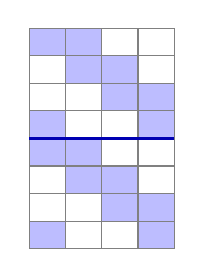
\begin{tikzpicture}[x=.46cm,y=.35cm]
\foreach \i in {0,...,7} {
  \foreach \j in {0,...,3} {
    \pgfmathtruncatemacro{\firstcol}{mod(\i,4)}
    \pgfmathtruncatemacro{\nextcol}{mod(\i+1,4)}
    \ifnum\j=\firstcol \fill[blue!26] (\j,-\i) rectangle +(1,-1); \fi
    \ifnum\j=\nextcol \fill[blue!26] (\j,-\i) rectangle +(1,-1); \fi
    \draw[gray] (\j,-\i) rectangle +(1,-1);
  }
}
\draw[very thick,blue!70!black] (0,-4) -- (4,-4);
\end{tikzpicture}
\caption{Las dos columnas elegidas en cada fila del rectángulo, ilustrado con cuatro columnas. Cada fila contiene dos celdas elegidas y cada columna cuatro. La línea gruesa separa las dos copias del patrón cíclico.}\label{fig:rectangle}
\end{figure}

\section{Asignación de excepcionales y déficits exactos por bloques}\label{sec:block-routing}

Podemos dividir los vértices ordinarios de un corte en bloques correspondientes. Aunque un color deje el mismo total de vértices libres en ambos lados, los conteos pueden diferir dentro de un bloque. Asignar un excepcional a un bloque usa un ordinario del lado opuesto y cambia esa diferencia en uno.

Fijemos un color. Escribimos \(u_j,v_j\) para los conteos de ordinarios libres a la izquierda y a la derecha del bloque \(j\) y ponemos \(\delta_j=u_j-v_j\). Sean \(X,Y\) los conjuntos de excepcionales libres de cada lado. Cada excepcional tiene un conjunto de bloques elegibles. Si \(p^A_j,p^B_j\) cuentan los excepcionales de izquierda y derecha asignados a \(j\), quedan \(u_j-p^B_j\) y \(v_j-p^A_j\) ordinarios en sus respectivos lados. Estas cantidades son iguales exactamente cuando
\[
 p^B_j-p^A_j=\delta_j.
\]
El balance total de vértices libres da \(\sum_j\delta_j=|Y|-|X|\). Para un conjunto \(S\) de bloques, sea \(L(S)\) el número de excepcionales izquierdos cuyos bloques elegibles están todos en \(S\), y \(R(S)\) el de excepcionales derechos con algún bloque elegible en \(S\). Escribimos \(\delta(S)=\sum_{j\in S}\delta_j\).

Por ejemplo, supongamos que hay dos bloques con \(\delta_1=1\) y \(\delta_2=-1\). Se pueden satisfacer las hipótesis de anchura de abajo tomando \((u_1,v_1)=(\theta+2,\theta+1)\) y \((u_2,v_2)=(\theta+1,\theta+2)\), con umbral \(\theta\) en ambos bloques. Si el excepcional izquierdo solo puede usar el bloque~1 y el derecho solo el bloque~2, entonces \(L(\{1\})=1\) y \(R(\{1\})=0\). El corte del primer bloque tiene una diferencia de \(1-0+1=2\). Permitir al excepcional derecho usar ambos bloques reduce la mayor diferencia a \(1\). Permitir también al izquierdo usar ambos bloques la reduce a \(0\), pues ahora podemos enviar al izquierdo al bloque~2 y al derecho al bloque~1. El Teorema~\ref{thm:block-deficit} convierte esas diferencias de corte en déficits exactos de emparejamiento.

\begin{lemma}[Asignación por bloques]\label{lem:block-assignment}
Supongamos que hay balance total. Existe una asignación elegible con \(p^B_j-p^A_j=\delta_j\) en cada bloque si y solo si
\[
 \delta(S)\le R(S)-L(S)
 \qquad\text{para todo conjunto \(S\) de bloques.}
 \tag{A}\label{eq:block-assignment}
\]
Si además se exige \(p^B_j\le c_j\) para enteros no negativos dados \(c_j\), la condición necesaria y suficiente es
\[
 \delta(S)\le R(T)-L(S)+\sum_{j\in S\setminus T}c_j
 \qquad\text{para todo par \(S,T\) de conjuntos de bloques.}
 \tag{C}\label{eq:block-capacity}
\]
\end{lemma}

\begin{proof}
Para \eqref{eq:block-assignment}, construimos una red con un nodo por cada bloque y por cada excepcional. Sus arcos de capacidad uno van de los excepcionales izquierdos a los bloques elegibles y de los bloques a los excepcionales derechos elegibles. Las entradas netas prescritas son \(-1\) en los excepcionales izquierdos, \(1\) en los derechos y \(-\delta_j\) en el bloque \(j\). Un flujo entero con esas demandas da los conteos buscados. Por el teorema de factibilidad de Gale, la demanda en el complemento de cada corte debe ser a lo sumo la capacidad que entra en él \cite{Gale}.

Fijemos el conjunto \(S\) de nodos de bloques del lado de la fuente. El aporte de los bloques a la demanda en el complemento es \(-\delta(S^c)\). Un excepcional izquierdo en el complemento aporta \(-1\). Del lado de la fuente aporta el negativo del número de sus bloques elegibles fuera de \(S\), una vez descontada la capacidad entrante. Al maximizar sobre el lado que contiene a este excepcional obtenemos \(0\) si todos sus bloques elegibles están en \(S\), y \(-1\) en otro caso. Del mismo modo, el aporte máximo de un excepcional derecho es \(0\) si puede usar un bloque en \(S\), y \(1\) en otro caso. La diferencia máxima entre demanda y capacidad entrante es por tanto
\[
 -\delta(S^c)-|X|+L(S)+|Y|-R(S)
 =\delta(S)+L(S)-R(S).
\]
Esto prueba la primera afirmación.

Para \eqref{eq:block-capacity}, introducimos dos copias \(j^-,j^+\) de cada bloque. Los excepcionales reales izquierdos solo usan la primera, y los derechos solo la segunda. Para cada \(j\) añadimos \(c_j\) excepcionales izquierdos elegibles para cualquiera de las dos copias. Prescribimos diferencias \(\delta_j-c_j\) y \(0\) en la primera y segunda copia, respectivamente. En la segunda, la cantidad añadida debe ser \(p^B_j\), y los otros \(c_j-p^B_j\) añadidos van a la primera. La primera copia fuerza \(p^B_j-p^A_j=\delta_j\). La construcción funciona en ambos sentidos. Al aplicar \eqref{eq:block-assignment} a los bloques duplicados se obtiene la condición con dos conjuntos. Un corte con las primeras copias de \(S\) y las segundas de \(T\) ya descontó \(c_j\) de la demanda para cada \(j\in S\). Los excepcionales añadidos quedan forzados a entrar en el corte precisamente para \(j\in S\cap T\), lo que cancela esas capacidades. Las capacidades restantes en \eqref{eq:block-capacity} corresponden a bloques con \(j^-\) en el corte y \(j^+\) fuera.
\end{proof}

Para el paso de emparejamiento, supongamos que cada excepcional elegible tiene en su bloque una reserva ponderada suficiente para Hall después de gastar a lo sumo \(k-1\) copias cruzadas previas en cada vértice. Las cotas por columna cuentan todos los excepcionales elegibles de ese lado del bloque. En particular, se aplican a cualquier conjunto de excepcionales asignados allí. Por Hall emparejamos a los excepcionales asignados con ordinarios, por separado para los excepcionales izquierdos y derechos. Los dos emparejamientos son disjuntos porque usan conjuntos opuestos de excepcionales.

Supongamos también que cada bloque \(j\) tiene un umbral ordinario \(\theta_j\). Cuando dos subconjuntos ordinarios no vacíos \(S,T\) de lados opuestos de ese bloque cumplen \(|S|+|T|>\theta_j\), algún vértice de \(S\cup T\) tiene al menos \(k\) copias cruzadas originales hacia el subconjunto opuesto. Entonces dos conjuntos ordinarios libres del mismo tamaño, al menos \(\theta_j\), se pueden emparejar a pesar del gasto anterior. Si el emparejamiento falla, Hall da dos conjuntos no vacíos sin aristas residuales y cuya suma de tamaños excede el tamaño libre común. Se habrían gastado todas las copias entre ellos, contra la cota de \(k\) copias.

\begin{corollary}[Factorización con capacidades por bloque]\label{cor:block-factorization}
Sea \(M\) un multigrafo regular con un corte equilibrado. Supongamos que las aristas internas tienen un coloreo propio con \(k\) colores y que cada color deja igual número de vértices libres en ambos lados. Usemos las reservas ponderadas locales y los umbrales ordinarios recién descritos. Para cada color exijamos \(u_j\ge\theta_j\) e impongamos \eqref{eq:block-capacity} con \(c_j=u_j-\theta_j\). Entonces los colores internos se pueden completar con copias cruzadas disjuntas y \(M\) tiene una 1-factorización.
\end{corollary}

\begin{proof}
El Lema~\ref{lem:block-assignment} da una asignación que respeta \(c_j\). Tras emparejar a los excepcionales, los conteos ordinarios del bloque \(j\) son iguales y \(u_j-p^B_j\ge\theta_j\). El paso de emparejamiento ordinario completa el color. Después de completar todos los colores internos, factorizamos el residuo bipartito regular como en el Teorema~\ref{thm:factor}.
\end{proof}

La mayor diferencia de corte mide el costo de incumplir la condición de balance. La hipótesis de anchura del siguiente teorema permite aplicar el paso de emparejamiento ordinario con cualquier asignación elegible, incluso si un bloque recibe todos los excepcionales del lado opuesto.

\begin{theorem}[Déficit exacto]\label{thm:block-deficit}
Fijemos un color con conteos libres totales iguales. Supongamos que cada excepcional tiene al menos un bloque elegible, que valen las reservas de Hall y los umbrales ordinarios anteriores, y que \(u_j\ge\theta_j+|Y|\) y \(v_j\ge\theta_j+|X|\) para cada bloque \(j\). Entre las completaciones parciales que cubren a todos los excepcionales y respetan sus asignaciones y la partición ordinaria en bloques, el mínimo número de vértices sin emparejar en cada lado es
\[
 d=\max_S\bigl(\delta(S)-R(S)+L(S)\bigr).
 \tag{E}\label{eq:block-deficit}
\]
Los mínimos de todos los colores se pueden alcanzar con copias cruzadas disjuntas. Cambiar las listas de elegibilidad de a lo sumo \(r\) excepcionales cambia el valor de \eqref{eq:block-deficit} en a lo sumo \(r\).
\end{theorem}

\begin{proof}
Para cualquier asignación elegible, la suma de las partes positivas de los desbalances después de asignar es al menos \(\delta(S)-R(S)+L(S)\) para todo \(S\). Un emparejamiento dentro de los bloques deja sin emparejar al menos esa suma de desbalances positivos en la izquierda. Esto prueba la cota inferior.

Los cortes del conjunto vacío y del conjunto completo tienen diferencia cero. Añadimos \(d\) excepcionales por lado, todos elegibles para todos los bloques. Para cada conjunto no vacío y propio de bloques, el lado derecho de \eqref{eq:block-assignment} aumenta en \(d\). Las desigualdades del vacío y del conjunto completo siguen cumpliéndose. El Lema~\ref{lem:block-assignment} asigna todos los excepcionales. Luego descartamos los añadidos. Quedan a lo sumo \(d\) unidades de desbalance positivo, pues en la derecha se añadieron \(d\) excepcionales en total.

Las reservas ponderadas cubren a los excepcionales reales con esta asignación. El lado ordinario menor que queda en cada bloque tiene al menos \(\theta_j\) vértices. Recortamos el lado mayor a ese tamaño y aplicamos el paso de emparejamiento ordinario. El conteo sin emparejar alcanza la cota inferior. Esto funciona después de gastar hasta \(k-1\) copias previas por vértice, de modo que al repetir por colores se alcanzan todos los mínimos. Por último, cambiar la lista de un excepcional altera \(R(S)\) o \(L(S)\) en a lo sumo uno para cada corte. La misma estimación vale para el máximo.
\end{proof}

\section{Completación simultánea en una reserva espectral}\label{sec:spectral-reserve}

Primero usamos las reservas ponderadas de Hall para emparejar a los excepcionales libres de cada color. Luego emparejamos los ordinarios que quedan libres mediante dos conjuntos disjuntos de copias cruzadas. Uno da emparejamientos parciales para toda la paleta. El otro da recorridos que reparan esos emparejamientos sin volver a usar una copia.

\subsection{El lema de reparación}

En un bloque ordinario, los dos lados físicos tienen tamaño \(N\). Para cada color \(i\), los conjuntos libres de ambos lados tienen igual tamaño y \(M_i\) es un emparejamiento inicial entre ellos. Escribimos \(X_i,Y_i\) para los vértices libres que \(M_i\) deja sin cubrir, y \(A_i^-,B_i^-\) para todos los vértices físicos que \(M_i\) deja sin cubrir. Estos últimos conjuntos incluyen los vértices no disponibles en el color.

\begin{lemma}[Reparación en una reserva espectral]\label{lem:spectral-repair}
Sea \(R\) un grafo bipartito simple \(d\)-regular sobre los dos lados físicos, con \(d>0\). Cada arista de \(R\) representa una copia cruzada reservada para reparaciones. Los emparejamientos iniciales usan copias fuera de \(R\) y son disjuntos dos a dos en copias. Supongamos que la matriz de biadyacencia normalizada \(P\) de \(R\) tiene norma de operador a lo sumo \(\sigma<1\) en los vectores de media cero. Sea \(h\ge1\) tal que \(\sigma^h\le1/(2N)\) y pongamos \(\ell=2h+1\).

En cada color, cada vértice físico tiene a lo sumo \(\rho d\) vecinos de reserva en el conjunto opuesto \(A_i^-\) o \(B_i^-\) que quedó sin cubrir. Cada vértice físico pertenece a lo sumo a \(t\) de los conjuntos libres que quedaron sin cubrir en su propio lado. Si hay \(k\) colores y
\[
 3(\ell-1)\rho\le\frac12,\qquad
 6\ell\,\frac{2t+(\ell-2)k\rho}{d}+6(\ell-1)^2\rho\le\frac{4}{27},
 \tag{P}\label{eq:spectral-repair}
\]
entonces se pueden emparejar todos los conjuntos ordinarios libres usando copias cruzadas disjuntas dos a dos de los emparejamientos iniciales y de \(R\).
\end{lemma}

\begin{proof}
Para cada color extendemos \(M_i\) a una biyección \(\pi_i\) del lado físico izquierdo al derecho, emparejando \(X_i\) con \(Y_i\) y emparejando por separado los vértices no disponibles. Cada par \(x,\pi_i(x)\) con \(x\in X_i\) es una solicitud. Identificamos los estados derechos con las coordenadas izquierdas mediante \(\pi_i^{-1}\). La matriz de transición sobre esas coordenadas es \(K_i(u,v)=P(u,\pi_i(v))\). Un recorrido para la solicitud \(x\) empieza en \(x\), da \(\ell\) pasos de reserva y está condicionado a terminar en la coordenada \(x\).

Tanto \(K_i\) como \(K_i^{\mathsf T}\) conservan las constantes y contraen los vectores de media cero por un factor a lo sumo \(\sigma\). Una masa puntual centrada tiene norma euclidiana a lo sumo uno, así que cada entrada para un tramo de al menos \(h\) pasos difiere de \(1/N\) en a lo sumo \(\sigma^h\). Por consiguiente, cada entrada está entre \(1/(2N)\) y \(3/(2N)\). Invertir la lista de estados y sustituir \(K_i\) por \(K_i^{\mathsf T}\) conserva el producto de las probabilidades de transición y la masa en los extremos que lo normaliza. Así se obtiene la misma ley condicionada a los extremos al leer el recorrido al revés. En cualquier paso de reserva, el tramo estrictamente anterior o el estrictamente posterior tiene longitud al menos \(h\). Al leer desde el extremo con el tramo más corto, todo evento determinado hasta el paso elegido aumenta su probabilidad por un factor a lo sumo \(3\) al condicionar por los extremos. Esto se sigue de dividir la cota superior \(3/(2N)\) para el tramo no examinado por la cota inferior \(1/(2N)\) para la masa en los extremos.

Una coordenada intermedia es admisible cuando representa un par de \(M_i\). En cada posición intermedia, uno de los dos tramos adyacentes tiene longitud al menos \(h\). Antes de condicionar, un paso hacia esa posición llega a una coordenada prohibida con probabilidad a lo sumo \(\rho\), por la cota de vecinos de reserva en \(B_i^-\) en el recorrido directo o en \(A_i^-\) en el inverso. El condicionamiento por los extremos eleva la cota a \(3\rho\). La primera desigualdad de \eqref{eq:spectral-repair} y la cota de la unión dan probabilidad condicional al menos \(1/2\) de que todas las coordenadas intermedias sean admisibles. Restringirnos a esos recorridos aumenta las cotas siguientes por un factor adicional de a lo sumo dos.

Para contar cuánto puede usarse una copia de reserva, iniciamos un recorrido sin condicionar desde cada \(x\in X_i\). Después del primer paso, la masa total en cada coordenada es a lo sumo \(\rho\), pues a lo sumo \(\rho d\) vecinos de \(A_i^-\) pueden enviarle masa \(1/d\). La matriz de transición conserva esa cota superior porque sus columnas suman uno. Los recorridos inversos respetan la misma cota al partir de \(Y_i\). En un paso interior de reserva tomamos la dirección con el tramo largo sin examinar. La masa total que atraviesa una copia fija en ese paso y color es a lo sumo \(\rho/d\) antes de condicionar. Después de ambos condicionamientos es a lo sumo \(6\rho/d\). En un paso extremo, solo las solicitudes que empiezan o terminan en el vértice físico correspondiente pueden usar la copia, así que la cota en toda la paleta es \(6t/d\) en cada extremo. Para una arista del emparejamiento anterior contamos solo solicitudes de su color. En cada posición intermedia la cota superior es \(6\rho\), por el mismo argumento con la masa en la coordenada contraída. Sumando sobre las posiciones se acotan las probabilidades de usar un recurso al menos una vez, sumadas sobre todas las solicitudes,
\[
 \mu_R=\frac{6\bigl(2t+(\ell-2)k\rho\bigr)}{d}
 \qquad\text{y}\qquad
 \mu_M=6(\ell-1)\rho.
\]

Elegimos los recorridos independientemente, uno por solicitud. Para dos solicitudes distintas \(p,q\), el evento \(E_{pq}\) es que compartan una copia de reserva o una arista del emparejamiento anterior de su color común. Una cota de la unión sobre los recursos del recorrido de \(p\), seguida de un promedio sobre ese recorrido, da
\[
 \sum_{q\ne p}\Pr(E_{pq})\le\ell\mu_R+(\ell-1)\mu_M\le\frac{4}{27}.
\]
En el grafo de dependencias, dos eventos son adyacentes cuando se intersecan sus pares de solicitudes. Un evento es independiente de toda la colección de eventos cuyos pares evitan el suyo, pues las elecciones de base son independientes. Para un evento \(E_{pq}\) de probabilidad positiva ponemos \(x_{pq}=\tfrac94\Pr(E_{pq})\le1/3\). Dividimos sus vecinos en los que involucran a \(p\) y los restantes, que involucran a \(q\). En cada grupo la suma de los \(x\) es a lo sumo \(\tfrac94\cdot\tfrac4{27}=\tfrac13\). Cada grupo aporta un producto de \(1-x\) de al menos \(2/3\) por la cota \(\prod_j(1-x_j)\ge1-\sum_j x_j\). El producto sobre ambos grupos es al menos \(4/9\), y \(x_{pq}\cdot4/9=\Pr(E_{pq})\). El lema local asimétrico de Lovász~\cite{EL} da una elección de recorridos que evita todos los conflictos.

Para un color fijo, consideremos el grafo de aristas utilizables formado por su emparejamiento anterior y las copias de reserva de sus recorridos elegidos. Verificamos la desigualdad de Hall en las coordenadas contraídas. Para un conjunto \(S\) de coordenadas libres izquierdas, el emparejamiento anterior da los vecinos derechos \(S\setminus X_i\). Una solicitud en \(x\in S\cap X_i\) recorre desde \(x\) hasta \(x\). Su primer paso de reserva con llegada fuera de \(S\setminus X_i\) sale de \(S\). La llegada es su propio extremo sin emparejar o una coordenada emparejada. Estas llegadas son distintas para solicitudes distintas, pues los extremos sin emparejar se asignaron mediante una biyección y compartir una coordenada emparejada reutilizaría una arista del emparejamiento anterior. Así hay \(|S\cap X_i|\) vecinos derechos adicionales. Esto prueba la desigualdad de Hall para todo \(S\). Los emparejamientos resultantes solo usan las copias asignadas a sus respectivos colores. Dos colores pueden pasar por el mismo vértice físico, como en la Figura~\ref{fig:repair}.
\end{proof}

\begin{figure}[htbp]
\centering
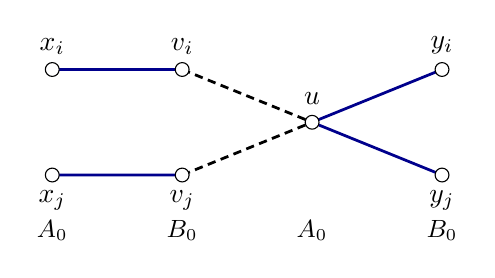
\begin{tikzpicture}[x=1.65cm,y=.67cm,
  vertex/.style={circle,draw,fill=white,inner sep=1.3pt,minimum size=5pt},
  reserve/.style={line width=1pt,blue!55!black},
  matched/.style={line width=1pt,densely dashed}]
  \coordinate (xi) at (0,1); \coordinate (xj) at (0,-1);
  \coordinate (vi) at (1,1); \coordinate (vj) at (1,-1);
  \coordinate (u) at (2,0);
  \coordinate (yi) at (3,1); \coordinate (yj) at (3,-1);
  \draw[reserve] (xi)--(vi) (xj)--(vj) (u)--(yi) (u)--(yj);
  \draw[matched] (vi)--(u) (vj)--(u);
  \foreach \name in {xi,xj,vi,vj,u,yi,yj} \node[vertex] at (\name) {};
  \foreach \name/\lab in {xi/x_i,vi/v_i,yi/y_i}
     \node[above=2pt] at (\name) {$\lab$};
  \foreach \name/\lab in {xj/x_j,vj/v_j,yj/y_j}
     \node[below=2pt] at (\name) {$\lab$};
  \node[above=3pt] at (u) {$u$};
  \foreach \col/\side in {0/$A_0$,1/$B_0$,2/$A_0$,3/$B_0$}
     \node[font=\small] at (\col,-2.05) {\side};
\end{tikzpicture}
\caption{Dos colores pueden pasar por el mismo vértice izquierdo \(u\). En el color \(i\), la arista discontinua \(v_i u\) pertenece al emparejamiento anterior y las dos aristas continuas son copias de reserva. El recorrido de abajo repara el color \(j\) con otras copias de reserva. Dentro de un color, un segundo recorrido por el mismo vértice emparejado reutilizaría su arista del emparejamiento anterior.}\label{fig:repair}
\end{figure}

\subsection{Un criterio de factorización mediante un \emph{nibble}}

Supongamos que los dos lados físicos de ordinarios tienen tamaño \(N\). Sea \(C\) un conjunto de copias cruzadas ordinarias disjunto de la reserva \(R\). Dados los conjuntos ordinarios libres \(F_i,G_i\), el hipergrafo de incidencia tiene un vértice por cada demanda izquierda \((i,x)\) con \(x\in F_i\), uno por cada demanda derecha \((i,y)\) con \(y\in G_i\) y uno por cada copia \(e\in C\). Cada uso elegible de una copia \(e=xy\) da la terna
\[
 \{(i,x),(i,y),e\}.
\]
La elegibilidad requiere \(x\in F_i\) e \(y\in G_i\). El grado de una demanda cuenta copias elegibles. El grado de una copia cuenta colores elegibles. Un cogrado puede exceder uno solo para dos demandas de lados opuestos en el mismo color, cuando hay copias paralelas elegibles entre sus extremos.

Usamos la estimación del \emph{nibble} de Keevash~\cite[Sección~3.1]{KeevashII}, en la forma de pesos iguales que se deriva de Ehard, Glock y Joos~\cite{EGJ}. Fijemos \(0<\delta<1\). Para \(\Delta\) suficientemente grande en función de \(\delta\), sea el hipergrafo de incidencia de grado máximo a lo sumo \(\Delta\), cogrados a lo sumo \(\Delta^{1-\delta}\) y todos los grados de demanda al menos \((1-\eta)\Delta\), donde \(0\le\eta<1\). Si el número de ternas y el número de pruebas son cada uno a lo sumo \(\exp(\Delta^{(\delta/450)^2})\), existe un emparejamiento que deja masa sin cubrir a lo sumo
\[
 B(z)=\max\left\{(\eta+\Delta^{-\delta/450})z,\frac{3\Delta^\delta}{1-\eta}\right\}
 \label{eq:nibble-error}\tag{N}
\]
en cada prueba elegida con soporte en las demandas, pesos en \([0,1]\) y masa total \(z\).

\begin{theorem}[Factorización a partir de reservas ponderadas y un \emph{nibble}]\label{thm:hybrid-completion}
Fijemos \(0<\delta<1\). Sea \(M\) un multigrafo \(D\)-regular con un corte equilibrado e igual número de ordinarios a cada lado. Sus aristas internas tienen un coloreo propio con \(k\le D\) colores, que deja el mismo número de vértices libres en los dos lados para cada color.

Designemos copias cruzadas separadas para las filas excepcionales en ambas orientaciones, un conjunto ordinario \(C\) y una reserva ordinaria simple \(d\)-regular \(R\), con \(d>0\). En cada par, la suma de copias designadas es a lo sumo su multiplicidad en \(M\). Las dos orientaciones de filas excepcionales tienen los siguientes certificados ponderados de Hall. Para una fila \(x\), sea \(\eta_x\ge0\) su costo por copia gastada. Su peso en una columna ordinaria está entre cero y \(\eta_x\) por la multiplicidad designada en ese par. El peso total de una columna es a lo sumo una cota positiva común. En cada color, una fila excepcional libre tiene en las columnas ordinarias libres peso al menos esa cota más \((k-1)\eta_x\). Las estimaciones suficientes \eqref{eq:rowx} y \eqref{eq:rowy} dan estos certificados al medirlas sobre las copias designadas.

Supongamos que después de cualquier elección factible de emparejamientos entre excepcionales y ordinarios que cubra todos los excepcionales libres y respete las copias designadas, se cumplen las siguientes condiciones sobre los conjuntos ordinarios libres \(F_i,G_i\) restantes.
\begin{enumerate}
\item Para algún \(\Delta\) suficientemente grande en función de \(\delta\) y algún \(0\le\eta<1\), el hipergrafo de incidencia de \(C\) satisface las cotas de grado y cogrado de \eqref{eq:nibble-error}. Tanto su número de ternas como \(2N(k+1)\) son a lo sumo \(\exp(\Delta^{(\delta/450)^2})\).
\item La matriz normalizada de \(R\) tiene norma a lo sumo \(\sigma<1\) sobre vectores de media cero. Cada vértice físico tiene a lo sumo \(\beta d\) vecinos de reserva fuera del conjunto libre opuesto de cualquier color. Para un entero \(h\ge1\) con \(\sigma^h\le1/(2N)\), las cantidades
\[
 \ell=2h+1,\qquad t=B(k),\qquad \rho=\beta+B(d)/d
\]
satisfacen \eqref{eq:spectral-repair}.
\end{enumerate}
Entonces los \(k\) colores internos se extienden a emparejamientos perfectos con copias cruzadas disjuntas dos a dos y \(M\) tiene una 1-factorización.
\end{theorem}

\begin{proof}
El argumento ponderado de Hall del Teorema~\ref{thm:factor} cubre los vértices excepcionales. En cada orientación, los a lo sumo \(k-1\) colores anteriores pueden reducir el peso de una fila en a lo sumo \((k-1)\eta_x\). Las cotas restantes de filas y columnas dan la desigualdad de Hall. Las dos orientaciones cubren conjuntos disjuntos de vértices en cada color, pues cada una une un excepcional con un ordinario. Retiran el mismo número de vértices en cada lado del corte, por lo que \(|F_i|=|G_i|\).

Usamos dos clases de pruebas con indicadores en el \emph{nibble}. En cada vértice físico contamos sus demandas a lo largo de la paleta, a lo sumo \(k\). Para cada color y vértice físico contamos las demandas libres opuestas entre sus vecinos de reserva, a lo sumo \(d\). Hay \(2N(k+1)\) pruebas. El emparejamiento de ternas da emparejamientos iniciales \(M_i\) en \(C\) con copias físicas distintas en todos los colores. Las primeras pruebas acotan por \(B(k)\) el número de conjuntos libres sin cubrir que contienen a cualquier vértice. Las segundas acotan por \(B(d)\) el número de vecinos ordinarios que quedan sin cubrir en cada vértice y color. Al añadir los vecinos ya no disponibles resulta la cota \(\beta d+B(d)=\rho d\) para los conjuntos sin cubrir del Lema~\ref{lem:spectral-repair}.

El lema completa los emparejamientos ordinarios. Sus copias y las que usaron los emparejamientos de excepcionales respetan las capacidades designadas en cada par físico. Junto con las aristas internas dan \(k\) emparejamientos perfectos disjuntos. El residuo tiene grado \(D-k\) y contiene solo copias cruzadas, por lo que se factoriza por el teorema de Hall.
\end{proof}

El teorema de Hall da los emparejamientos de excepcionales a partir de las cotas de filas y columnas. Los grados de demanda ordinarios y las vecindades de reserva dependen de los vértices que usen esos emparejamientos. Una cota de pérdidas válida para cada emparejamiento factible permite aplicar las estimaciones ordinarias a la elección que da Hall. Si cada lado pierde a lo sumo \(s\) ordinarios, cada vértice de un conjunto simple de copias pierde a lo sumo \(s\) vecinos en el lado opuesto. Eliminar ternas elegibles conserva las cotas superiores de grados de copia y cogrados. Usamos estas cotas en la rejilla que sigue.

\subsection{Una familia dispersa de rejillas fuera del criterio de rectángulos}\label{sec:sparse-reserve-example}

Fijemos enteros \(b\ge1\) y \(q\ge12\) par. Cada lado tiene \(N=bq^2\) ordinarios en una rejilla de \(q\) por \(q\) con \(b\) vértices por celda. Numeramos filas y columnas de \(0\) a \(q-1\). Dos vértices opuestos son adyacentes en el soporte de la rejilla cuando comparten fila o columna. Cada par del soporte tiene una copia en \(C\) y otra en \(R\), de modo que ambos conjuntos tienen grado \(d=b(2q-1)\). Sobre vectores constantes en cada celda, la matriz del soporte es \(b(J_q\otimes I_q+I_q\otimes J_q-I_{q^2})\), donde \(J_q\) es la matriz de unos. El valor propio sobre las constantes es \(d\). Si exactamente una de las funciones de coordenada tiene suma cero, el valor propio es \(b(q-1)\). Si ambas tienen suma cero, es \(-b\). En vectores de suma cero en cada celda, la matriz es cero. Por tanto, la norma de la reserva normalizada sobre el espacio de media cero es \((q-1)/(2q-1)<1/2\).

Ponemos \(d\) copias en un par interno izquierdo y en uno derecho. Los pares usan las columnas \(0,1\) en la fila \(0\) de la izquierda y en la fila \(q/2\) de la derecha. Una copia de cada par va en cada uno de \(k=d\) colores. Los ordinarios internamente libres se emparejan a través del corte por coordenadas iguales donde es posible. Las dos coordenadas izquierdas restantes en la fila \(q/2\) se emparejan con las dos derechas restantes en la fila \(0\) en sus columnas respectivas. Cada par de esta biyección recibe \(d\) copias de relleno.

Hay \(r=\lfloor\sqrt q\rfloor\) excepcionales por lado, emparejados a través del corte. Para cada par excepcional \(x,y\) elegimos dos pares de relleno \(u_L,u_R\) de coordenadas iguales en la fila \(q/2+1\), con las \(2r\) coordenadas distintas entre los excepcionales. Esto es posible pues \(2r\le q\). En cada coordenada elegida, las \(d\) copias de relleno se sustituyen por \(d\) de \(u_Ly\) y \(d\) de \(xu_R\). Ponemos también \(d\) copias en \(xy\). Las sustituciones conservan cada grado ordinario, que es \(3d\) por los dos conjuntos de la rejilla y las copias internas o de relleno. Un excepcional tiene dos vecinos ordinarios de multiplicidad \(d\) y su pareja excepcional de multiplicidad \(d\), así que también tiene grado \(3d\).

\paragraph{Los parámetros del criterio híbrido.}
Cada fila excepcional puede dar peso \(d\) a sus dos vecinos ordinarios, con la misma cota de columna y costo uno. Esos vecinos están inicialmente libres en todos los colores y cada columna pertenece a una sola fila en cada orientación. Después de cualquier emparejamiento factible de los excepcionales, cada lado ordinario libre tiene tamaño \(N-r-2\). Un vértice físico pierde a lo sumo \(r+2\) vecinos en cada conjunto de la rejilla. El hipergrafo de incidencia tiene entonces grado máximo a lo sumo \(d\), cogrado a lo sumo uno y grados de demanda al menos \(d-r-2\). El número de ternas es a lo sumo \(kNd\) y el de pruebas es \(2N(k+1)\), ambos polinomiales en \(q\).

Tomamos \(\Delta=k=d\), \(\delta=1/4\) y \(\eta=\beta=(r+2)/d\). Con \(b\) fijo, \(\eta=O(d^{-1/2})\) y
\[
 \frac{B(d)}{d}
 =\max\left\{\eta+d^{-1/1800},\,\frac{3d^{-3/4}}{1-\eta}\right\}
 =O(d^{-1/1800}).
\]
Así, tanto \(t/d\) como \(\rho\) son \(O(d^{-1/1800})\). Tomando \(h=\lceil\log_2(2N)\rceil\) se obtiene \(\ell=O(\log N)\). Como \(k=d\), ambos lados izquierdos de \eqref{eq:spectral-repair} están acotados por \(O((\log N)^2d^{-1/1800})=o(1)\). Esto da la aplicación asintótica del Teorema~\ref{thm:hybrid-completion}.

\begin{corollary}[Factorización de la rejilla y separación del criterio de rectángulos]\label{cor:sparse-grid}
Para todo \(b\ge1\) y \(q\ge12\) par, el multigrafo recién construido tiene una 1-factorización. Tiene \(d=\Theta(\sqrt N)\) vecinos ordinarios cruzados distintos por vértice ordinario y \(r=\Theta(N^{1/4})\) excepcionales por lado para \(b\) fijo. El criterio de rectángulos del Teorema~\ref{thm:factor} falla para toda paleta interna admisible en este corte.
\end{corollary}

\begin{proof}
El umbral explícito proviene de los pares de relleno. En cada una de las \(d\) rondas usamos una copia de cada arista interna. En la primera coordenada modificada para \(x,y\), emparejamos \(u_L\) con \(y\) y \(x\) con \(u_R\), usando copias nuevas en cada ronda. La segunda coordenada modificada para cada par de excepcionales queda sin cubrir en ambos lados. La llamamos un hueco. Un hueco puede intercambiar su relleno ausente con cualquier vecino de la rejilla cuyo relleno diagonal sigue intacto. Al excluir las cuatro coordenadas de extremos internos y las \(2r\) coordenadas modificadas quedan al menos \(d-(2r+4)\) opciones en cada hueco.

Mostramos que los intercambios se pueden programar siempre que
\[
 r\le m_0=\left\lceil\frac d2\right\rceil
 \qquad\text{y}\qquad
 \left\lfloor\frac d2\right\rfloor\ge 2r+4.
\]
Cada hueco tiene entonces al menos \(m_0\) ayudantes elegibles. Elegimos exactamente \(m_0\) para cada hueco. Así obtenemos un grafo bipartito simple de grado \(m_0\) en cada hueco y a lo sumo \(r\le m_0\) en cada ayudante. Por el teorema de coloreo bipartito de aristas de K\H{o}nig, estos pares se dividen en \(m_0\) emparejamientos. Cada uno cubre todos los huecos y los ayudantes usados en una ronda son distintos. Para \(q\ge12\), tenemos \(q\ge2r+5\). Si \(r\le3\), esto se sigue de \(q\ge12\), y si \(r\ge4\), de \(q\ge r^2\). Como \(\lfloor d/2\rfloor\ge q-1\), ambas desigualdades valen para todo \(b\ge1\).

Duplicamos la programación, asignamos las dos ocurrencias a conjuntos distintos de copias de la rejilla y conservamos \(d\) de las \(2m_0\) rondas. Si un hueco en la coordenada \(z\) usa un ayudante en \(w\), su intercambio usa \(z_Lw_R\) y \(w_Lz_R\). Ambos pares existen porque compartir fila o columna es simétrico. Los intercambios de una ronda son disjuntos. El conjunto y los extremos de una copia identifican su hueco, su ayudante y su dirección. Cada hueco usa un ayudante dado a lo sumo una vez en cada conjunto, así que todas las copias de los intercambios son distintas. Los ayudantes no usados y los dos pares de relleno fuera de la diagonal usan copias separadas de sus rellenos en cada ronda. Esto da \(d\) emparejamientos perfectos disjuntos que contienen las copias internas. El residuo es \(2d\)-regular y bipartito, de modo que se factoriza.

Para la separación, sea \(S\) la primera mitad izquierda de las filas y \(T\) la segunda mitad derecha. Sus tamaños suman \(N\). En ambas direcciones, cada vértice de este rectángulo ve \(bq/2\) vértices de la otra mitad a través de su columna y usa dos copias de la rejilla para cada uno. Las copias de relleno en coordenadas iguales y los dos rellenos de la segunda mitad izquierda a la primera mitad derecha aportan cero al rectángulo. Así, todo vértice tiene \(bq<d\) copias al conjunto opuesto. Un coloreo interno propio requiere al menos \(d\) colores porque cada par interno tiene \(d\) copias paralelas. El rectángulo excede el umbral \(N-r-2a\) del Teorema~\ref{thm:factor}, y las copias por vértice son menos que el tamaño de cualquier paleta admisible. El soporte cruzado ordinario es exactamente el de la rejilla, pues los rellenos fuera de la diagonal comparten columna. Con \(b\) fijo, las expresiones de \(N,d,r\) dan los órdenes de crecimiento indicados.
\end{proof}

La rejilla separa el criterio de rectángulos de la factorización en el corte dado. El umbral explícito \(q\ge12\) usa el emparejamiento de relleno para programar intercambios deterministas. El Teorema~\ref{thm:hybrid-completion} usa los conjuntos de copias ordinarias y de reserva bajo sus hipótesis de grado y espectrales, que se cumplen para esta rejilla para todo \(q\) suficientemente grande con \(b\) fijo.


\section{Formalización}

El companion de formalización~\cite{WECRCompanion} identifica las pruebas en Lean de los diez resultados numerados. Se verifican en un solo proyecto bajo Lean 4.35.0-rc3. El enunciado formal del Teorema~\ref{thm:hybrid-completion} incluye un renombramiento inyectivo de los colores iniciales y demuestra que preserva el color de cada copia de arista interna. El desarrollo de la rejilla verifica los dos argumentos de la Sección~\ref{sec:sparse-reserve-example}. Las pruebas de recoloreo y de corte reutilizan Overfull Criteria, un desarrollo del autor~\cite{TraversoOverfull}. El companion indica las dependencias fijadas, los registros de verificación y el cálculo independiente con Certo para la Figura~\ref{fig:rectangle}.

\section*{Agradecimientos}

El autor está profundamente agradecido a su esposa María Paz y a sus hijos Lucas, Juan Cristóbal, Francisca, Raimundo y Benjamín por su amor, paciencia y apoyo.

\section*{Uso de inteligencia artificial y herramientas computacionales}

Se usó ChatGPT/Codex, de OpenAI, para explorar y verificar argumentos y preparar el manuscrito. Lean 4 y Mathlib se usaron para las pruebas identificadas en el companion. La prueba de coloreo bipartito de aristas usada para factorizar el residuo proviene de la formalización del artículo V del autor sobre Erdős~81~\cite{TraversoV}, que atribuye las pruebas heredadas de Lean a Aristotle, de Harmonic.

Certo~\cite{Certo} produjo el certificado matricial finito de la rejilla rectangular de la Figura~\ref{fig:rectangle}. El companion indica la especificación de la matriz, el certificado y el informe de verificación.

El autor conserva la responsabilidad por los argumentos, las citas, el código y la presentación. La autoría corresponde a la persona indicada en la portada.

\begin{thebibliography}{99}
\small

\bibitem{AB} G.~Ambrus and R.~Bozzai, Colorful vector balancing, \emph{Mathematika} \textbf{70} (2024), e12274. \href{https://doi.org/10.1112/mtk.12274}{doi:\,\nolinkurl{10.1112/mtk.12274}}.
\bibitem{Spencer} J.~Spencer, Balancing unit vectors, \emph{J. Combin. Theory Ser. A} \textbf{30} (1981), 349--350. \href{https://doi.org/10.1016/0097-3165(81)90033-9}{doi:\,\nolinkurl{10.1016/0097-3165(81)90033-9}}.
\bibitem{KLOS} D.~K\"uhn, A.~Lo, D.~Osthus and K.~Staden, The robust component structure of dense regular graphs and applications, \emph{Proc. Lond. Math. Soc.} \textbf{110} (2015), 19--56. \href{https://doi.org/10.1112/plms/pdu039}{doi:\,\nolinkurl{10.1112/plms/pdu039}}.
\bibitem{Haemers} W.~H. Haemers, Interlacing eigenvalues and graphs, \emph{Linear Algebra Appl.} \textbf{226--228} (1995), 593--616. \url{https://pure.uvt.nl/ws/files/996579/interlac.pdf}.
\bibitem{FFMYZ} A.~Ferber, B.~Frederickson, D.~Mao, L.~Yepremyan and Y.~Zhu, Regular bipartite decompositions of pseudorandom graphs, \emph{J. Combin. Theory Ser. B} \textbf{179} (2026), 270--292. \href{https://doi.org/10.1016/j.jctb.2026.04.004}{doi:\,\nolinkurl{10.1016/j.jctb.2026.04.004}}.


\bibitem{BKLS}
P.~N. Balister, A.~V. Kostochka, H.~Li and R.~H. Schelp,
Balanced edge colorings,
\emph{J. Combin. Theory Ser. B} \textbf{90} (2004), 3--20.
\href{https://doi.org/10.1016/S0095-8956(03)00073-X}{doi:\,\nolinkurl{10.1016/S0095-8956(03)00073-X}}.

\bibitem{CariolaroFu}
D.~Cariolaro and H.-L. Fu,
Covering graphs with matchings of fixed size,
\emph{Discrete Math.} \textbf{310} (2010), 276--287. \url{https://ir.lib.nycu.edu.tw/bitstream/11536/13011/1/000273169900010.pdf}.


\bibitem{CMS}
G.~Chen, J.~McDonald and S.~Shan,
Towards the Overfull Conjecture II,
preprint, 2026.
\href{https://arxiv.org/abs/2607.02270v1}{arXiv:2607.02270v1}.

\bibitem{Gale}
D. Gale, A theorem on flows in networks,
\emph{Pacific J. Math.} \textbf{7} (1957), 1073--1082.
\href{https://doi.org/10.2140/pjm.1957.7.1073}{doi:\,\nolinkurl{10.2140/pjm.1957.7.1073}}.

\bibitem{GK}
R.~Gajjala and A.~Khan,
Asymptotically Optimal Weighted Edge Colorings via Local Bin Packing,
preprint, 2026.
\href{https://arxiv.org/abs/2611.03190}{arXiv:2611.03190}.

\bibitem{McDiarmid}
C.~J.~H. McDiarmid,
The solution of a timetabling problem,
\emph{J. Inst. Math. Appl.} \textbf{9} (1972), 23--34.
\href{https://doi.org/10.1093/imamat/9.1.23}{doi:\,\nolinkurl{10.1093/imamat/9.1.23}}.

\bibitem{NashWilliams}
C.~St.~J.~A. Nash-Williams,
Amalgamations of almost regular edge-colourings of simple graphs,
\emph{J. Combin. Theory Ser. B} \textbf{43} (1987), 322--342. \url{https://www.sciencedirect.com/science/article/pii/0095895687900086}.


\bibitem{PlantholtShan}
M.~J. Plantholt and S.~Shan,
On the Multigraph Overfull Conjecture,
\emph{J. Graph Theory} \textbf{109} (2025), 226--236.
\href{https://doi.org/10.1002/jgt.23221}{doi:\,\nolinkurl{10.1002/jgt.23221}}.

\bibitem{Shan}
S.~Shan,
The overfull conjecture on graphs of odd order and large minimum degree,
\emph{J. Graph Theory} \textbf{106} (2024), 322--351. \href{https://doi.org/10.1002/jgt.23077}{doi:\,\nolinkurl{10.1002/jgt.23077}}.

\bibitem{SY}
A.~Shioura and M.~Yagiura,
A fast algorithm for computing a nearly equitable edge coloring with balanced conditions,
\emph{J. Graph Algorithms Appl.} \textbf{14} (2010), 391--407.
\href{https://doi.org/10.7155/jgaa.00213}{doi:\,\nolinkurl{10.7155/jgaa.00213}}.

\bibitem{BFU}
A.~Z. Broder, A.~M. Frieze and E.~Upfal,
Existence and construction of edge-disjoint paths on expander graphs,
\emph{SIAM J. Comput.} \textbf{23} (1994), 976--989.
\href{https://doi.org/10.1137/S0097539792232021}{doi:\,\nolinkurl{10.1137/S0097539792232021}}.

\bibitem{EGJ}
S.~Ehard, S.~Glock and F.~Joos,
Pseudorandom hypergraph matchings,
\emph{Combin. Probab. Comput.} \textbf{29} (2020), 868--885.
\href{https://arxiv.org/abs/1907.09946}{arXiv:1907.09946}.

\bibitem{KeevashII}
P.~Keevash, The existence of designs II,
preprint, 2018.
\href{https://arxiv.org/abs/1802.05900}{arXiv:1802.05900}.

\bibitem{EL}
P.~Erd\H{o}s and L.~Lov\'asz,
Problems and results on 3-chromatic hypergraphs and some related questions,
in \emph{Infinite and Finite Sets}, Colloq. Math. Soc. J\'anos Bolyai \textbf{10},
North-Holland, Amsterdam, 1975, 609--627.


\bibitem{Certo}
J.~P. Traverso Gianini, \emph{Certo: computational tools with verifiable certificates}, version 0.40.0. Commit \texttt{df0ec25178a6}. \url{https://github.com/jtraverso/certo-math}.

\bibitem{TraversoV}
J.~P. Traverso Gianini,
\emph{Colorability and realizability defects in resource-dominated packing relaxations}, Preprint 1.0, 2026.
\url{https://github.com/jtraverso/erdos-81-chordal-clique-partitions/tree/papers-v-vi-notes-preprint-1.0/preprints/PAPER_V}.

\bibitem{TraversoOverfull}
J.~P. Traverso Gianini, \emph{Overfull Criteria}, desarrollo en Lean 4.
Registro de Palomar PALOMAR-2026-11-08-000004.
\url{https://github.com/jtraverso/overfull-criteria}.

\bibitem{WECRCompanion}
J.~P. Traverso Gianini,
\emph{Companion de formalización de Recoloreo ponderado de aristas y 1-factorización a través de un corte}, Preprint 1.0, 2026.
\url{https://github.com/jtraverso/weighted-edge-recoloring/releases/download/preprint-1.0/WECR_FORMALIZATION_COMPANION_v1.0_es.pdf}.

\end{thebibliography}
\end{document}
